\documentclass{article}

\usepackage{mathtools}
\usepackage[utf8]{inputenc}
\usepackage{amsmath}
\usepackage{amssymb}
\usepackage{graphicx}
\usepackage{bm}
\usepackage{enumitem}
\usepackage{textcomp}
\usepackage{amsthm}
\DeclarePairedDelimiter\ceil{\lceil}{\rceil}
\DeclarePairedDelimiter\floor{\lfloor}{\rfloor}

\usepackage[margin=1in]{geometry}
\setlength\parindent{0pt}
\setlength{\parskip}{5px}

\newtheorem{lemma}{Lemma}

\newcommand\at[2]{\left.#1\right|_{#2}}
\newcommand{\p}[2]{\frac{\partial #1}{\partial #2}}
\newcommand{\pp}[2]{\frac{\partial^2 #1}{\partial #2^2}}
\newcommand{\hes}[3]{\begin{pmatrix}
\frac{\partial^2 #1}{\partial #2 \partial #2} & \frac{\partial^2 #1}{\partial #2 \partial #3} \\
\frac{\partial^2 #1}{\partial #3 \partial #2} & \frac{\partial^2 #1}{\partial #3 \partial #3}
\end{pmatrix}}
\newcommand{\abs}[1]{\left| #1 \right|}
\newcommand{\paren}[1]{\left(#1\right)}
\newcommand{\brac}[1]{\left[#1\right]}
\newcommand{\R}{\mathbb{R}}
\newcommand{\half}{\frac{1}{2}}
\newcommand{\st}{\text{ s.t. }}
\newcommand{\vv}[2]{\begin{pmatrix}#1\\#2\end{pmatrix}}
\newcommand{\vvv}[3]{\begin{pmatrix}#1\\#2\\#3\end{pmatrix}}
\DeclareMathOperator*{\argmax}{arg\,max}
\DeclareMathOperator*{\argmin}{arg\,min}

\begin{document}

\title{MA3236 AY1819 Sem 1 Answers}
\author{Lim Li}
\maketitle

\subsection*{Question 1}

By KKT first order necessary condition, we have:

\[\nabla f(\bar{x}) + \lambda \begin{pmatrix}
1 \\ \vdots \\ 1
\end{pmatrix} + \mu^T \begin{pmatrix}
-1 \\ \vdots \\ -1
\end{pmatrix} = 0\]
Where $\mu$ is a vector such that $\mu \geq 0$, and $\mu_i = 0$ if $\bar{x}_i \neq 0$ ($x_i \geq 0$ is not active).

Hence, we consider the $j$-th coordinate:

\[\delta_j + \lambda - \mu_j = 0\]

Hence, we can choose the scalar $\kappa = -\lambda$, then
\[\delta_j + \lambda - \mu_j = 0 \implies \delta_j + \lambda \geq 0 \implies \delta_j \geq \kappa\]
\[\mu_i = 0 \text{ if } \bar{x}_i \neq 0 \implies (\mu_i)\bar{x}_i = 0 \implies (\delta_j + \lambda)\bar{x}_i = 0\]

Hence, $\kappa$ satisfies the conditions.

\subsection*{Question 2}

WLOG, we can assume $a=0$. This is because we can consider another function $\phi_2(x) = \phi(x+a)$ and $f_2(x) = f(x-a)$, so that $\phi_2 = f_2(x) + ||x||_2^2$.

WLOG, we can also assume $f(0)=0$, because we can consider another function $\phi_2(x) = \phi(x) - f(0)$.

Hence, it now suffices to prove that $\phi(x) = f(x) + ||x||_2^2$ is coercive given an extra condition that $f(0)=0$.

\begin{lemma}
For $x$ with $||x|| \geq 1$, $f(x) \geq ||x||f(\frac{x}{||x||})$
\end{lemma}
\begin{proof}
Since $f$ is convex, hence,
\[\frac{1}{||x||}f(x) + \frac{||x||-1}{||x||}f(0) \geq f(\frac{x}{||x||})\]
And since $f(0)=0$,
\[\therefore f(x) \geq ||x||f(\frac{x}{||x||})\]
\end{proof}

Hence, we can let $y := \argmin_{||x||=1} (f(x))$. Then, by the above lemma, for all $x$ with $||x||>1$, we have $f(x) \geq ||x||f(\frac{x}{||x||})$, and since $y$ minimizes $f(\frac{x}{||x||})$, hence, we have $f(x) \geq ||x||f(\frac{x}{||x||}) \geq ||x||f(y)$. Hence,

\[\phi(x) = f(x) + ||x||_2^2 \geq ||x||f(y) + ||x||_2^2\]

Which is quadratic in terms of $||x||$. Hence, as $||x|| \to \infty$, $\phi(x) \to \infty$.

\subsection*{Question 3}

\begin{enumerate}[label=(\alph*)]
\item Yes. The function is continuous. Since $(x_1-1)^2 + x_2^2 = 0$, hence $|x_1| \leq 100$, $|x_2| \leq 100$, which is bounded. The constraints are all closed as well. Hence, The feasible set is closed and bounded, which means the optimal solution exists.
\item
    Yes.
    
    \[\nabla g_1(x) = \vvv{2(x_1-1)}{2x_2}{0}\]
    \[\nabla g_2(x) = \vvv{0}{1}{-3x_3^2}\]
    
    \textbf{Case 1:} both $g_1$ and $g_2$ are non-zero
    
    Then, they have to be not linearly independent. Hence, there must exist some scalar such that $\nabla g_1(x) = k \nabla g_2(x)$
    \[\vvv{2(x_1-1)}{2x_2}{0} = k \vvv{0}{1}{-3x_3^2}\]
    Hence, $k=2x_2, x_1=1, x_3=0$.
    
    $x_3=0$ implies that $x_2=0$ (because of $g_2$). But $(1,0,0)$ is not feasible (because of $g_1$). Hence, all feasible points are regular for this case.
    
    \textbf{Case 2:} $\nabla g_1(x) = 0$
    
    Then, $x_1=1, x_2=0$. But this is not feasible (because of $g_1$). Hence, all feasible points are regular for this case.
    
\item
    \[\nabla f(x) = \vvv{2}{-1}{0}\]
    KKT first order necessary condition:
    \[\vvv{2}{-1}{0} + \lambda_1 \vvv{2(x_1-1)}{2x_2}{0} + \lambda_2 \vvv{0}{1}{-3x_3^2} = 0\]
    Hence, $\lambda_2=0$.
    \[\vv{2}{-1} + \lambda_1 \vv{2(x_1-1)}{2x_2} = 0\]
    Hence, $(x_1-1) = -2x_2$. Substitute this into $g_1$:
    \[(-2x_2)^2 + x_2^2 - 4 = 0 \implies x_2 = \pm \sqrt{\frac{4}{5}}\]
    \[x_1 = -2x_2+1 = \mp 2\sqrt{\frac{4}{5}} + 1\]
    
    The KKT points are $(\sqrt{\frac{4}{5}}, -2\sqrt{\frac{4}{5}} + 1, \sqrt[3]{-2\sqrt{\frac{4}{5}} + 1})$ and $(-\sqrt{\frac{4}{5}}, 2\sqrt{\frac{4}{5}} + 1, \sqrt[3]{2\sqrt{\frac{4}{5}} + 1})$.
\item
    Sub $(x_1,x_2) = (\sqrt{\frac{4}{5}}, -2\sqrt{\frac{4}{5}} + 1)$ into $f$:
    \[f(x)=4\sqrt{\frac{4}{5}}-1\]
    Sub $(x_1,x_2) = (-\sqrt{\frac{4}{5}}, 2\sqrt{\frac{4}{5}} + 1)$ into $f$:
    \[f(x)=-4\sqrt{\frac{4}{5}}-1\]
    The optimal is $-4\sqrt{\frac{4}{5}}-1$.
    
\end{enumerate}

\subsection*{Question 4}
If $d=0$, then $\phi(t) = 0$, a constant, which is clearly monotone increasing. Hence, WLOG, we can now assume that $d \neq 0$.

WLOG, we can assume $x=0$. This is because we can define another $f_2(y) = f(y+x)$ which is also convex, and $\phi(t) = \frac{f_2(td)-f_2(0)}{t}$.

WLOG, we can also assume $f(0)=0$. This is because we can define another $f_2(y) = f(y)-f(0)$ which is also convex, and $\phi(t) = \frac{f_2(td)}{t}$.

Hence, it now suffices to show that
\[\phi(t) = \frac{f(td)}{t}\]
is monotone increasing.

Let $t_1 > t_2 > 0$ be numbers in $\R_+$. Consider the two points at $t_1d$ and $0$. By convexity of $f$, we know that
\[\frac{t_2}{t_1} f(t_1 d) + \frac{t_1-t_2}{t_1} f(0) \geq f(t_2d)\]
Since $t_1 > t_2$, hence,
\[f(t_1 d) \geq \frac{t_2}{t_1} f(t_1 d) \geq f(t_2d)\]
Hence,
\[\phi(t_1) \geq \phi(t_2)\]
Hence, $\phi$ is monotone increasing.

\subsection*{Question 5}

\begin{figure}[h]
\centering
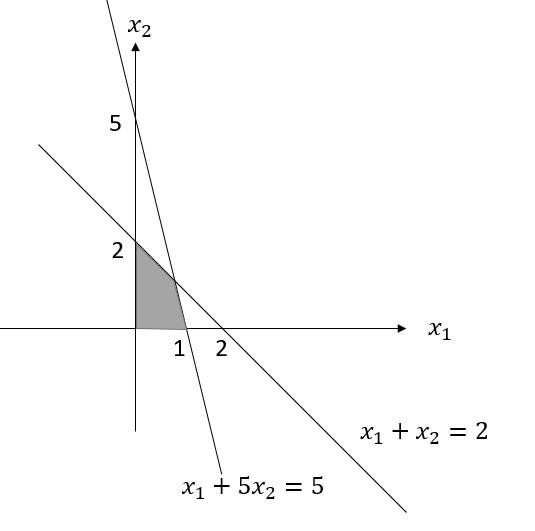
\includegraphics[width=5cm]{graph}
\caption{Plot of feasible area (shaded)}
\end{figure}

\[\nabla f(x) = \vv{2x_1 - x_2 - 2}{2x_2 - x_1 - 3}\]

First iteration:

Want to solve for $\min z(x) = f(\vv{5/4}{3/4}) + \nabla f(\vv{5/4}{3/4})^T(x-\vv{5/4}{3/4})$.
\begin{align*}
z(x) &= -\frac{57}{16} + \vv{-1/4}{-11/4}^T(x-\vv{5/4}{3/4}) \\
    &= -\frac{19}{16} - \vv{1/4}{11/4}^T (x)
\end{align*}

It suffices to check the four points $(0,0), (2,0), (0,1), (\frac{5}{4},\frac{3}{4})$, and we can find that $z(x)$ is minimum at $(0,1)$.

Then, direction $d = (0,1) - (\frac{5}{4},\frac{3}{4}) = (-\frac{5}{4},\frac{1}{4})$.

Now, we use line search to find $\min \{ \psi(t) = f((\frac{5}{4},\frac{3}{4}) + td) : 0 \leq t \leq 1\}$
\[x_1 = \frac{5}{4} - \frac{5}{4}t\]
\[x_2 = \frac{3}{4} + \frac{1}{4}t\]
\[f((x_1,x_2)) = (\frac{5}{4} - \frac{5}{4}t)^2 + (\frac{3}{4} + \frac{1}{4}t)^2 - (\frac{5}{4} - \frac{5}{4}t)(\frac{3}{4} + \frac{1}{4}t) - 2(\frac{5}{4} - \frac{5}{4}t) - 3(\frac{3}{4} + \frac{1}{4}t)\]
\[f((x_1,x_2)) = \frac{1}{16}[(5 - 5t)^2 + (3 + t)^2 - (5 - 5t)(3 + t) - 8(5 - 5t) - 3(3 + t)]\]

\[\psi'(t) = \frac{1}{16}[-5(5 - 5t) + (3 + t) + 5(3 + t) - (5 - 5t) + 40 - 3]\]
\[\psi'(t) = \frac{1}{16}[36t + 25]\]
Hence, $\psi(t)$ is minimum at $t = -\frac{25}{36}$. The point is updated from $(\frac{5}{4},\frac{3}{4})$ to $(\frac{5}{4},\frac{3}{4}) - \frac{25}{36}(-\frac{5}{4},\frac{1}{4}) = (\frac{305}{144}, \frac{83}{144})$.

Second iteration:

(i dunno how to continue, the numbers are very ugly)

\subsection*{Question 6}

\begin{enumerate}[label=(\roman*)]
\item
    \begin{align*}
    \theta(\lambda) &= \inf_{x \in X} \{f(x) + \lambda g(x) \} \\
        &= \inf_{x \in X} \{2x_1 +3x_2 + \lambda (x_1 + 3x_2 - 3) \}
    \end{align*}
    Dual problem:
    \[\max_{\lambda \in \R} \{\theta(\lambda)\}\]
\item To find $\inf_{x \in X} \{2x_1 +3x_2 + \lambda (x_1 + 3x_2 - 3) \}$, since the function is linear, it suffices to check the ``corners" of the set $X$, which are the points $(0,0),(1,0),(0,2)$.
    \begin{align*}
    \inf_{x \in X} \{2x_1 +3x_2 + \lambda (x_1 + 3x_2 - 3) \}
        &= \inf_{x \in X} \{(2+\lambda)x_1 +(3+3\lambda)x_2 \} - 3\lambda \\
        &= \inf_{x \in \{(0,0),(1,0),(0,2)\}} \{(2+\lambda)x_1 +(3+3\lambda)x_2 \} - 3\lambda \\
        &= \inf \{0, 2+\lambda, 6+6\lambda \} - 3\lambda \\
    \end{align*}
    \[
    \therefore \theta(\lambda)= \begin{cases}
    6+3\lambda & \text{if $\lambda \leq -1$}\\
    -3\lambda & \text{otherwise}
    \end{cases}
    \]
    We calculate the max of each case above:
    \[\max\{6+3\lambda | \lambda \leq -1\} = 3\]
    \[\max\{-3\lambda | \lambda \geq -1\} = 3\]
    Hence,
    \[\max_{\lambda \in \R} \theta(\lambda) = 3\]
\item Optimal solution is at $x^* = (0,1)$.

    Sub $\lambda = -1$ into $\inf_{x \in X} \{2x_1 +3x_2 + \lambda (x_1 + 3x_2 - 3) \}$, and we get
    \[\inf_{x \in X} \{x_1 + 3\}\]
    And we can see that the equation is minimum in the set $X$ when $x_1=0$. Substitute this into $g$ to get the optimal solution is $(0,1)$.
    
    We can then also verify that $f((0,1))=3$.
\item \[
    \partial \theta(\lambda)= \begin{cases}
    \{3\} & \text{if $\lambda < -1$}\\
    [-3,3] & \text{if $\lambda = -1$}\\
    \{-3\} & \text{if $\lambda > -1$}
    \end{cases}
    \]
\item 
    For $\lambda < -1$, the steepest direction is $1$.
    
    For $\lambda > -1$, the steepest direction is $-1$.
    
    For $\lambda = -1$, there is no ascent direction.
\end{enumerate}

\end{document}
